%============================================================
\section{Nombre: Zambullida.}\label{hab.zambullida}
\subsection{Descripción}
El enemigo se sumerge en el río, dejando a la vista su espalda, Una vez sumergido, el enemigo se desplaza del punto A al punto B a gran velocidad. La espalda del enemigo redice la cantidad de vida del jugador al hacer contacto con él.  
\subsection{Portador}
Zochitónal (ver apartado \ref{per:zochitonal}).
\subsection{Esquema}
			Ver figura \ref{fig:zambullida}.
			\begin{figure}
				\centering
				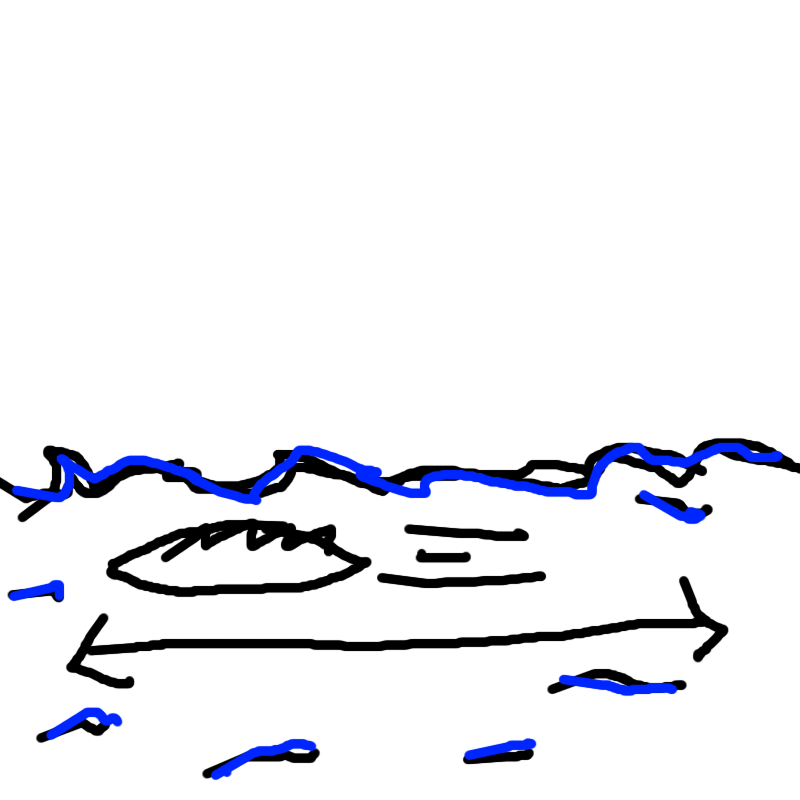
\includegraphics[height=0.2 \textheight]{Imagenes/zambullida}
				\caption{Zambullida.}
				\label{fig:zambullida}
			\end{figure}